\documentclass[11pt]{article}
\usepackage[margin=1in]{geometry}
\usepackage[T1]{fontenc}
\usepackage[utf8]{inputenc}
\usepackage{lmodern}
\usepackage{setspace}
\usepackage{graphicx}
\usepackage{booktabs}
\usepackage{hyperref}
\usepackage{float}
\setstretch{1.1}

\title{Supplementary Technical Note:\\Label-Conditioned and Diagnostic Error Analysis for Compiler-in-the-Loop SysML Generation}
\author{}
\date{}

\begin{document}
\maketitle

\begin{abstract}
This technical note extends the paper with multiple targeted analyses over 151 prompts and 4 models (604 runs). First, we perform a SysMBench label-conditioned analysis stratified by domain, key grammar label, and difficulty, including support-aware interpretation and subgroup comparisons of iterations-to-success. Second, because SysMBench uses line count as a difficulty proxy, we run an analogous generated-output analysis that relates final SysML line count to iterations-to-converge and reports both a global linear fit and model-wise average output length. Third, using SysIDE diagnostic outputs, we analyze error-family concentration (single-shot volume, cumulative volume, and prompt coverage), repair dynamics for top error families (completion curves), and persistence behavior when errors are not fixed immediately. Persistence is classified hierarchically as exact recurrence, template recurrence, or family-only churn. Together, these analyses characterize where repair burden concentrates, how quickly common error families resolve, and which failure modes persist through iterative correction.
\end{abstract}

\section{Experimental Context}
The analysis covers 151 unique prompts across four models (604 total model-prompt runs). Under iterative repair, eventual syntactic success is 100\% for all models, so the informative outcomes are first-shot pass, iterations-to-success, and diagnostic repair dynamics.

Difficulty labels are computed directly from ground-truth SysML size (line count): difficulty 1 for fewer than 30 lines, difficulty 2 for 30--59, difficulty 3 for 60--89, difficulty 4 for 90--119, and difficulty 5 for 120 or more lines. This is the exact binning logic used in SysMBench (\texttt{src/metrics/get\_difficult\_metrics.py}) and is used consistently throughout the label-conditioned analysis.

\begin{table}[h]
\centering
\caption{Overall campaign-level model outcomes (all prompts).}
\begin{tabular}{lccc}
\toprule
Model & First-shot pass (\%) & Eventual pass (\%) & Mean iterations-to-success \\
\midrule
Anthropic Claude Sonnet 4.6 & 82.781 & 100.000 & 1.225 \\
DeepSeek Reasoner & 41.060 & 100.000 & 1.974 \\
Mistral Large & 39.073 & 100.000 & 1.980 \\
OpenAI & 41.722 & 100.000 & 1.728 \\
\bottomrule
\end{tabular}
\end{table}

\section{Analysis Using SysMBench Labels}
This section uses the SysMBench label schema to identify where repair effort varies. The labels are not used as prompt inputs in this analysis; they are used to stratify outcomes after generation.

\subsection{Support and Interpretability}
Label support is strongly imbalanced and directly affects interpretability. We have 13 domains, 47 grammar labels, and 5 difficulty levels; however, most runs come from difficulty 1--2, and only a subset of grammar/domain categories have large support. Figure~\ref{fig:fig10} is therefore a required companion to all subgroup comparisons in this section.

\begin{figure}[H]
\centering
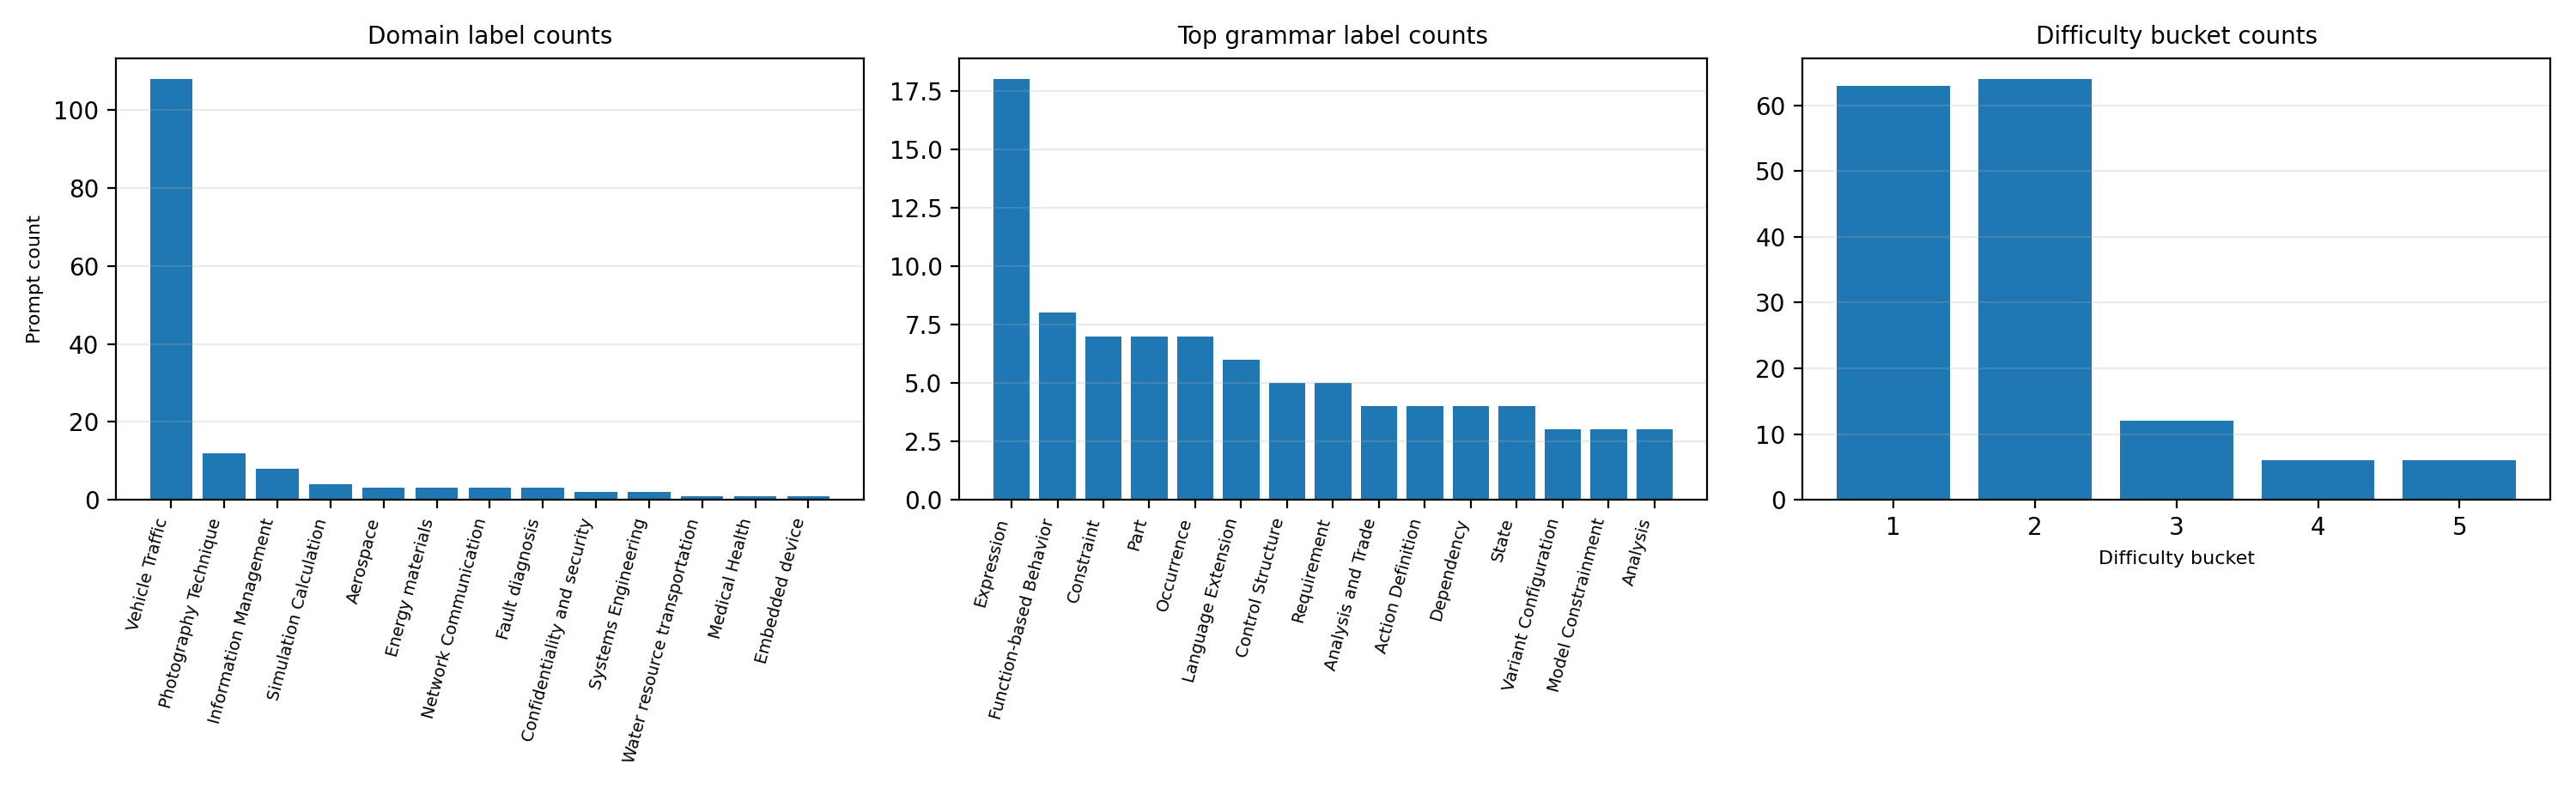
\includegraphics[width=\textwidth]{figures/fig10_label_sample_size_panels.png}
\caption{Support context for subgroup analysis (\texttt{fig10}).}
\label{fig:fig10}
\end{figure}

\subsection{Domain-Conditioned Repair Effort}
Figure~\ref{fig:fig03} shows mean iterations-to-success by domain and model. Averaged across models, domain means range from approximately 1.25 to 2.63 iterations. The highest means are observed in Systems Engineering (2.625), Medical Health (2.25), and Fault Diagnosis (2.00), while lower means appear in Embedded Device and Water Resource Transportation (both 1.25). These differences are meaningful, but the uncertainty is not uniform across domains due to unequal sample support.

\begin{figure}[H]
\centering
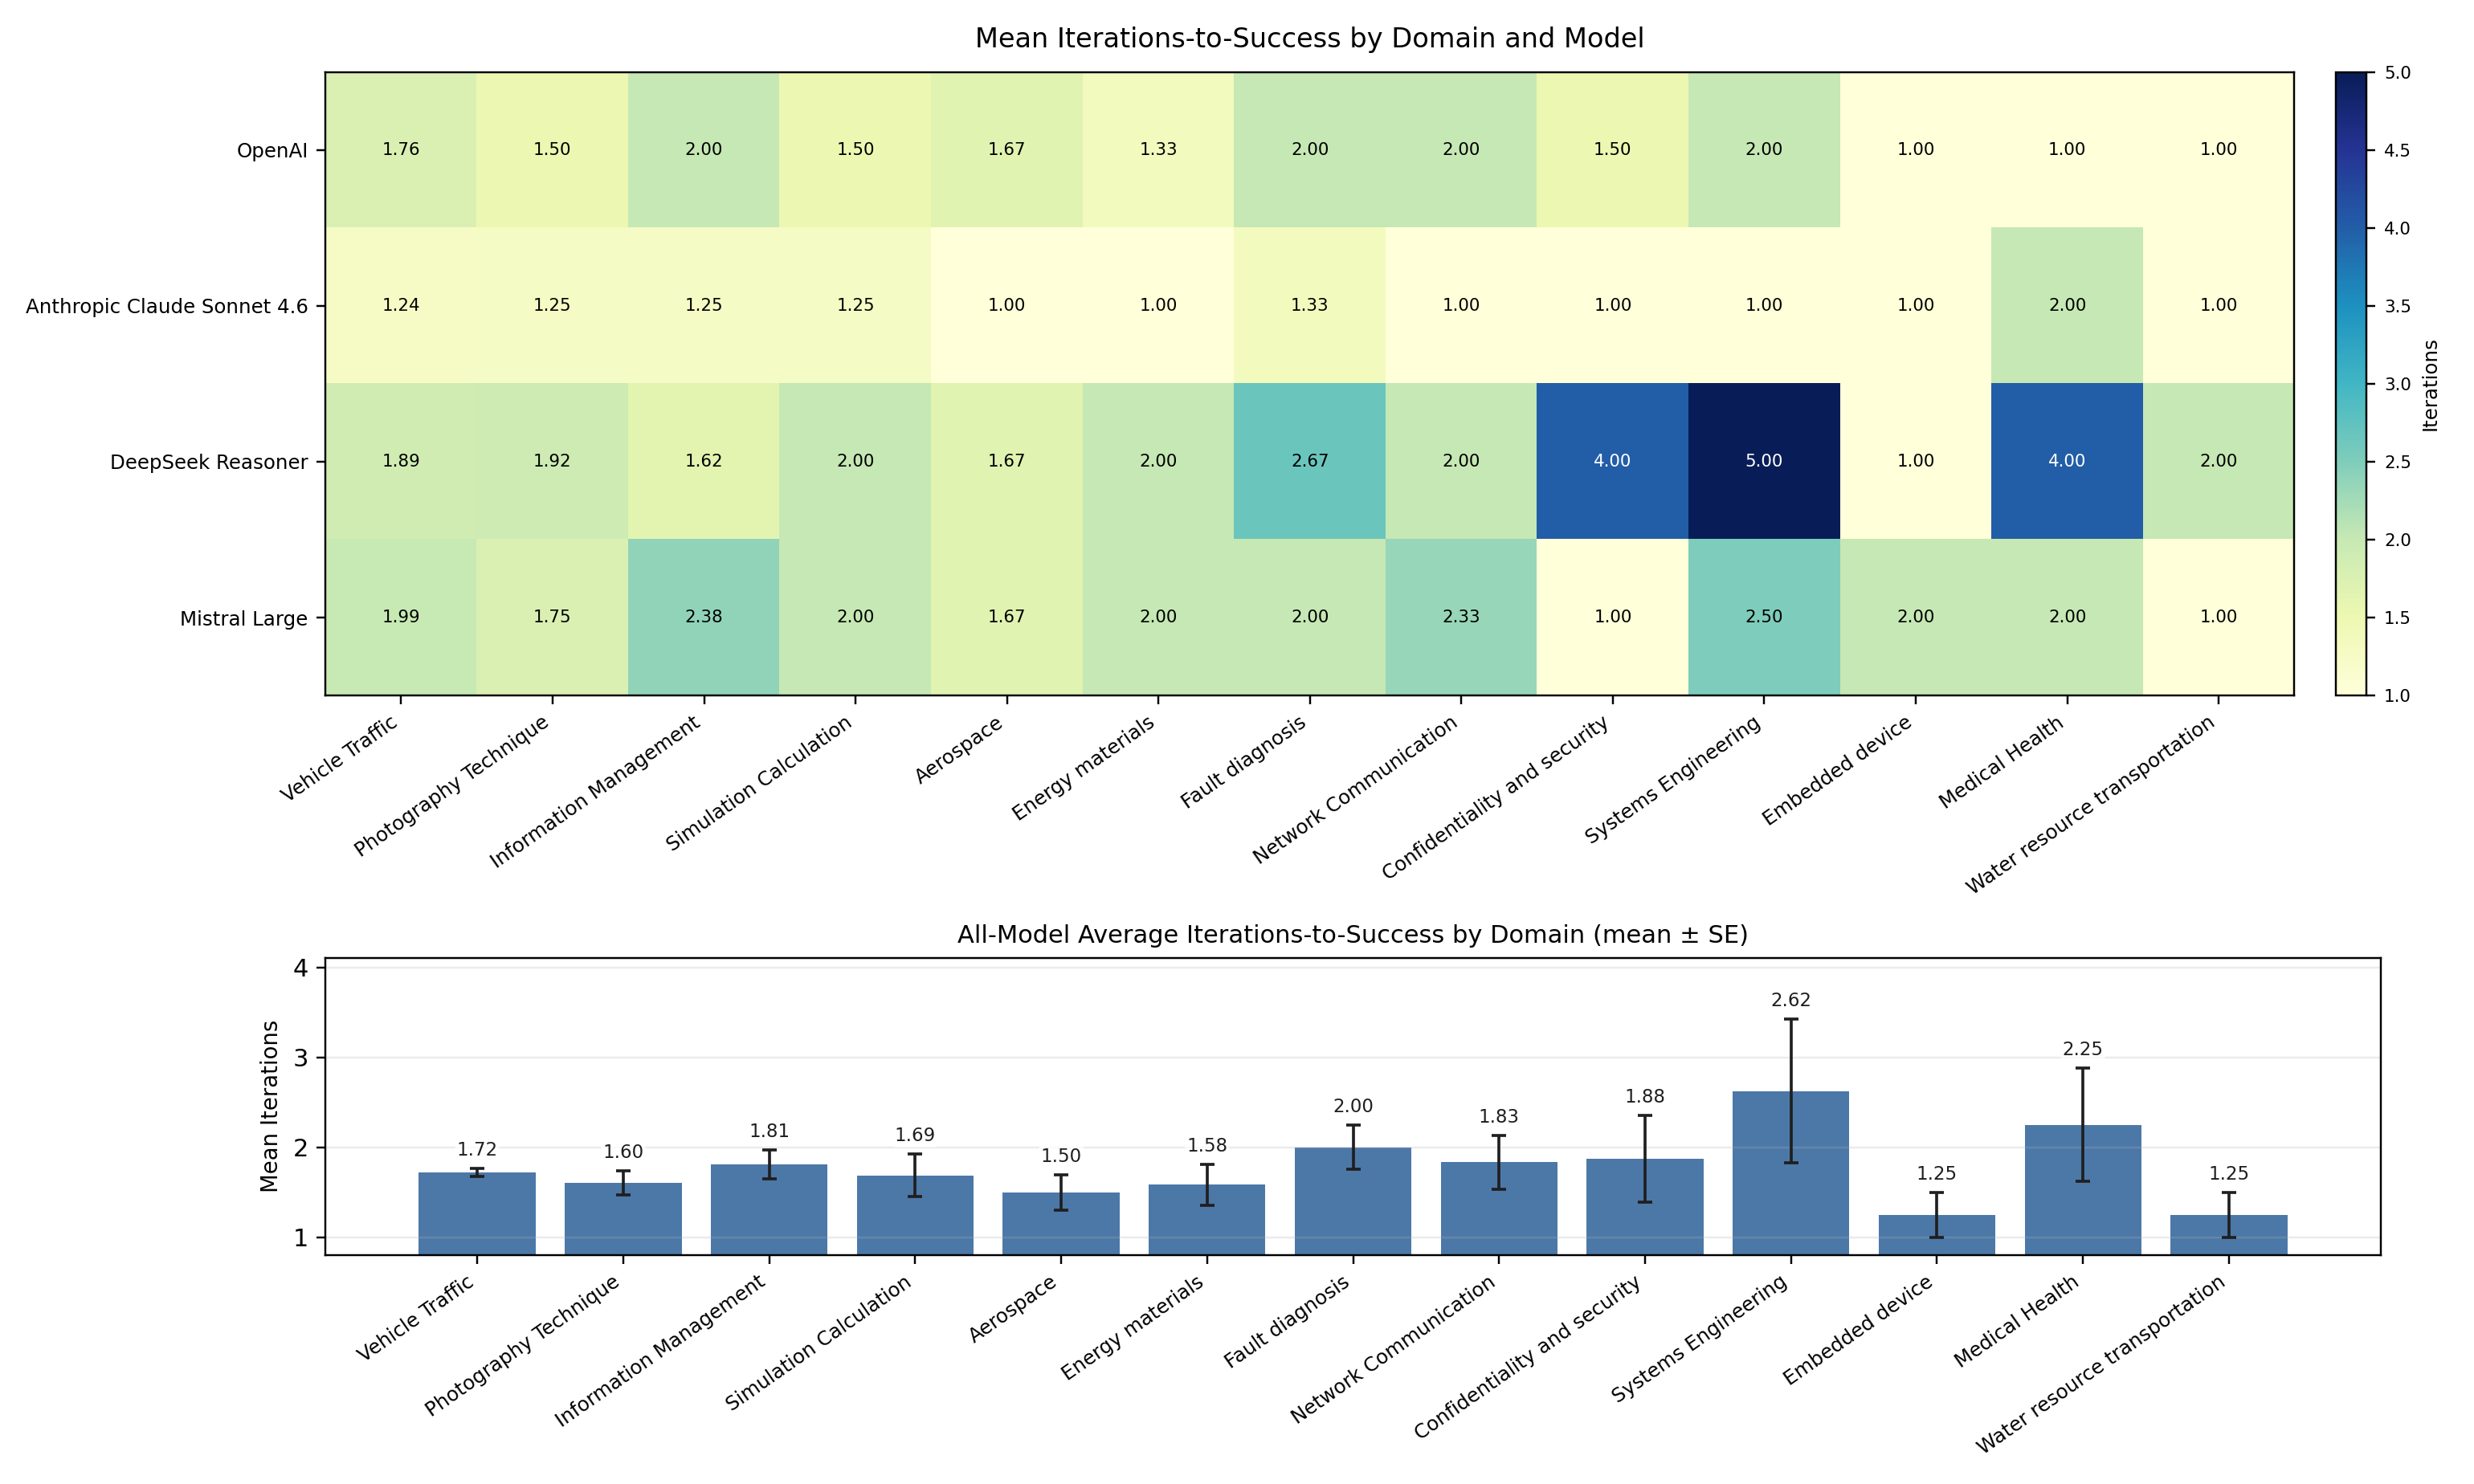
\includegraphics[width=\textwidth]{figures/fig03_domain_iterations_to_success_heatmap.png}
\caption{Mean iterations-to-success by domain and model (\texttt{fig03}).}
\label{fig:fig03}
\end{figure}

\subsection{Grammar-Conditioned Repair Effort}
Figure~\ref{fig:fig06} reports top-15 grammar labels by support. The top-15 cover 58.3\% of prompts (88/151), so this plot captures the majority regime while avoiding sparse-label noise. Within this set, Requirement (2.25 mean iterations), Analysis and Trade (2.062), and Language Extension (1.958) are associated with the highest average repair effort; Variant Configuration and Verification (both 1.333) are lower.

\begin{figure}[H]
\centering
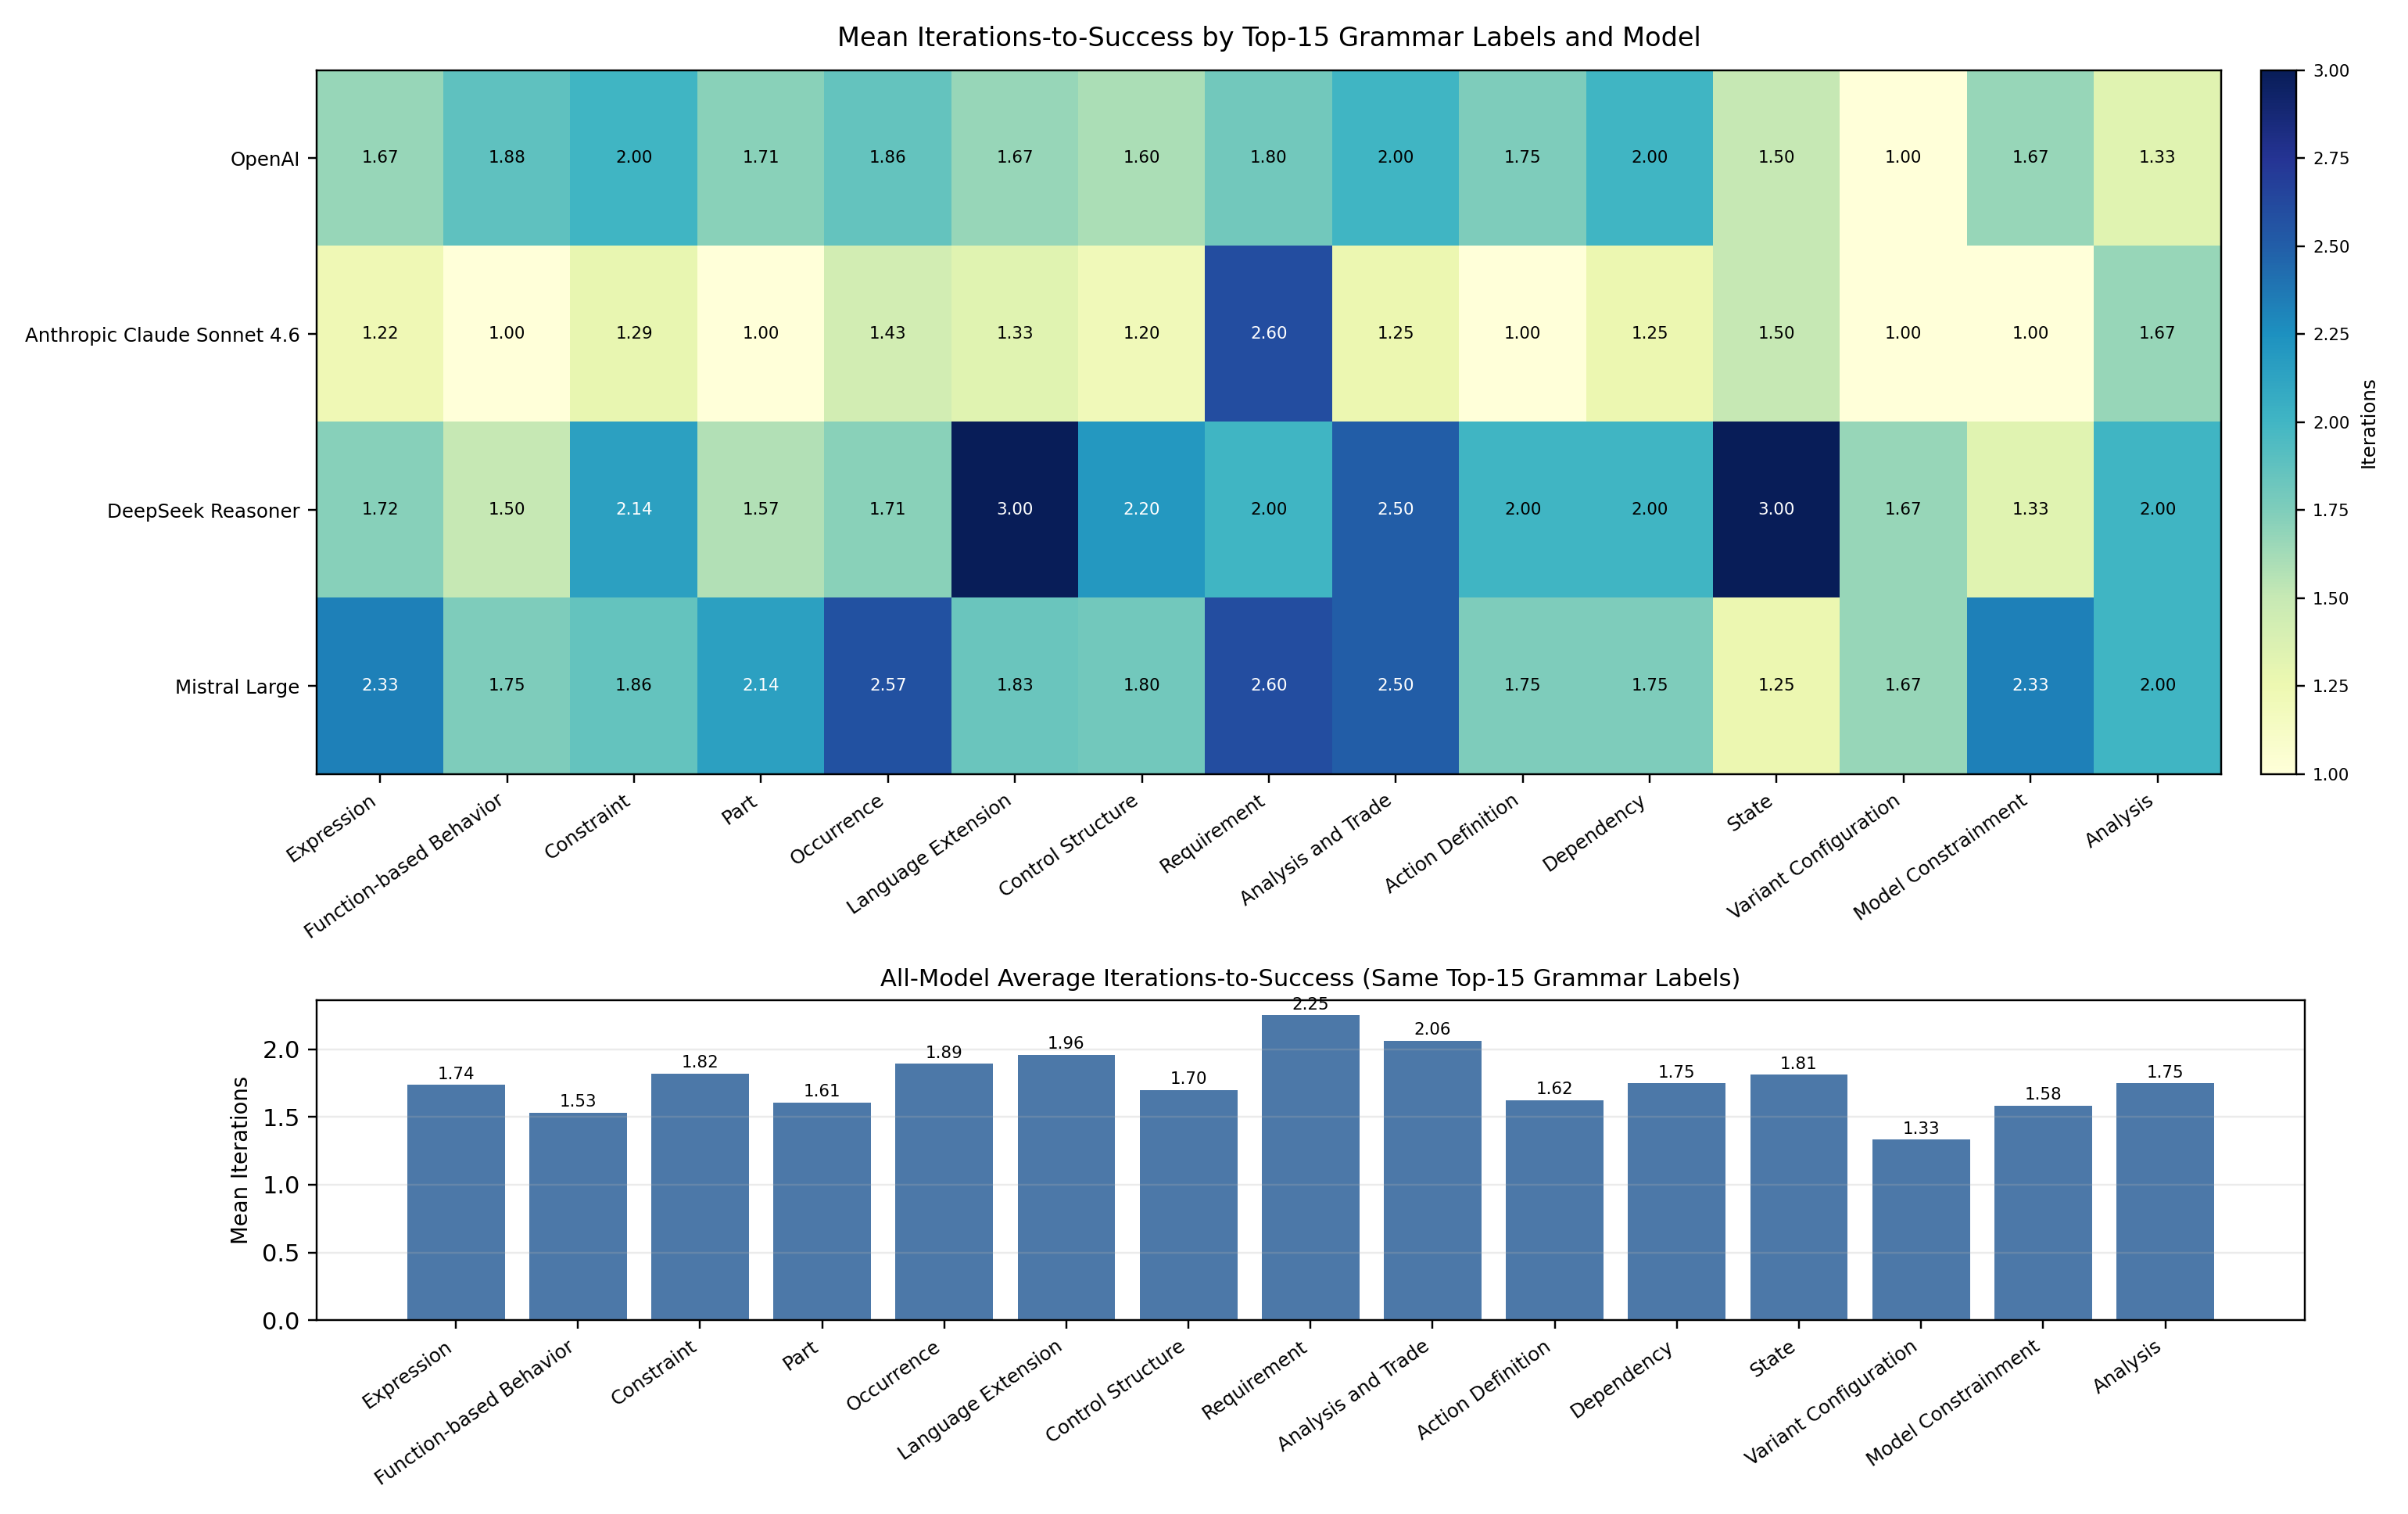
\includegraphics[width=\textwidth]{figures/fig06_grammar_topK_iterations_to_success_heatmap.png}
\caption{Top-15 grammar labels: model-wise and pooled iterations-to-success (\texttt{fig06}).}
\label{fig:fig06}
\end{figure}

\subsection{Difficulty Signal}
Figure~\ref{fig:fig09} evaluates difficulty versus iterations-to-success. The pooled means are: difficulty 1 = 1.766, difficulty 2 = 1.668, difficulty 3 = 1.938, difficulty 4 = 1.667, and difficulty 5 = 1.583. The combined trend panel in this figure shows a weak linear fit (\(R^2 \approx 0.183\)), indicating that the line-count-based difficulty label is informative but not strongly monotonic in this campaign.

\begin{figure}[H]
\centering
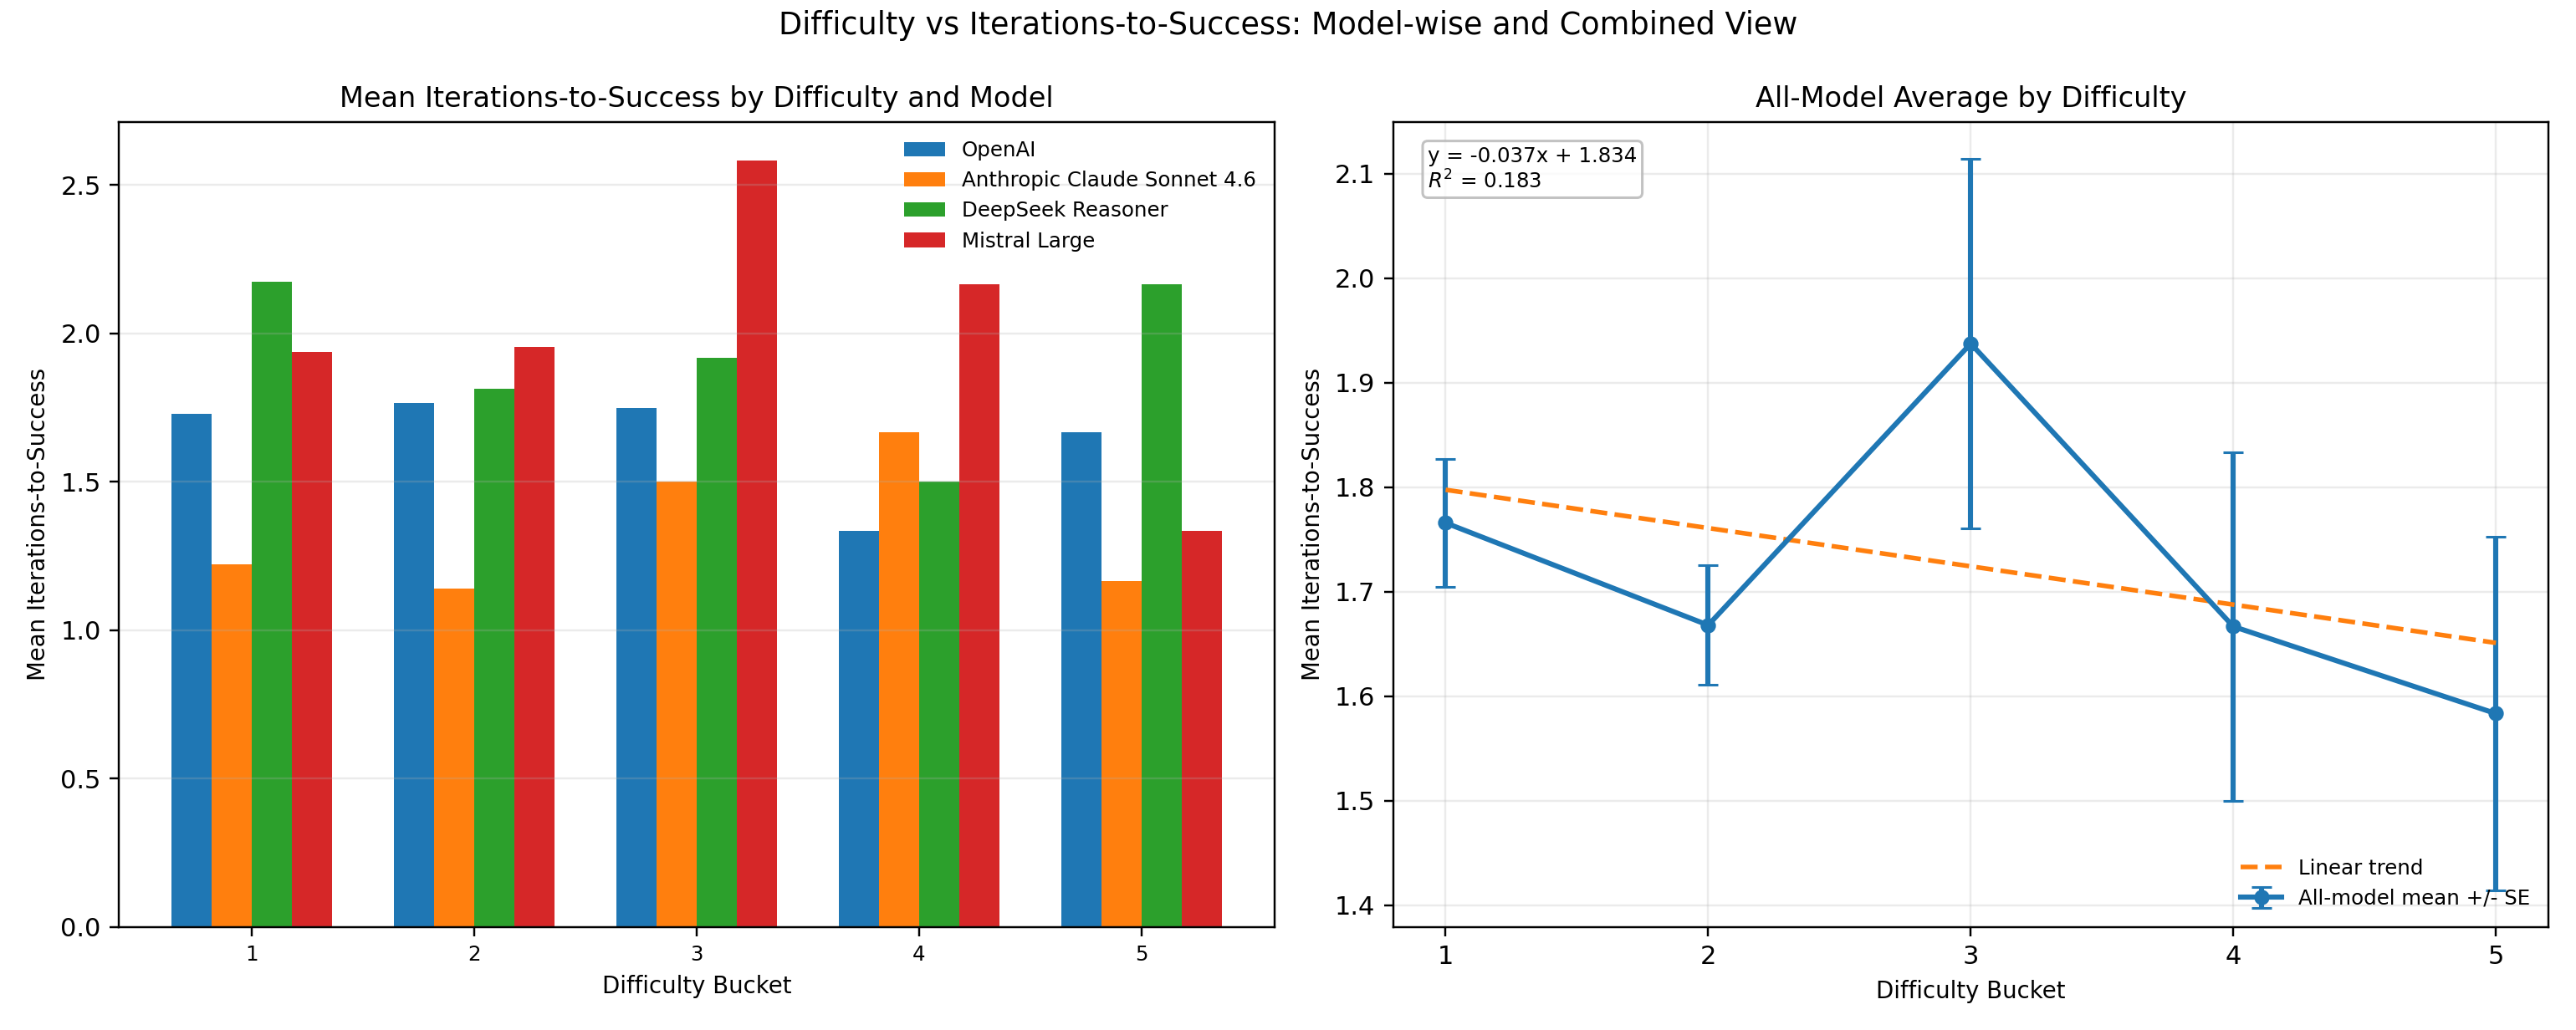
\includegraphics[width=\textwidth]{figures/fig09_difficulty_mean_iterations_to_success_grouped_bar.png}
\caption{Difficulty-conditioned repair effort with model split and pooled trend (\texttt{fig09}).}
\label{fig:fig09}
\end{figure}

\subsection{Analogous Analysis Using Generated SysML Size}
Because SysMBench uses line count as a proxy for difficulty, we also ran an analogous analysis on \emph{generated} SysML outputs: final output line count versus iterations-to-converge. Figure~\ref{fig:fig14} shows (left) the linear-scale scatter with global trendline and (right) average generated line count by model.

The linear fitted relationship remains weak (\(R^2 = 0.0011\), slope \(=0.00062\)), indicating that generated file length alone does not explain convergence iteration count in a meaningful way. The model-level panel shows that Anthropic produces substantially longer outputs on average than the other three models, yet this does not translate into a strong line-count-to-iteration relationship in the pooled scatter. This is consistent with Figure~\ref{fig:fig09}: convergence appears to depend more on error type/composition than on size alone.

\begin{figure}[H]
\centering
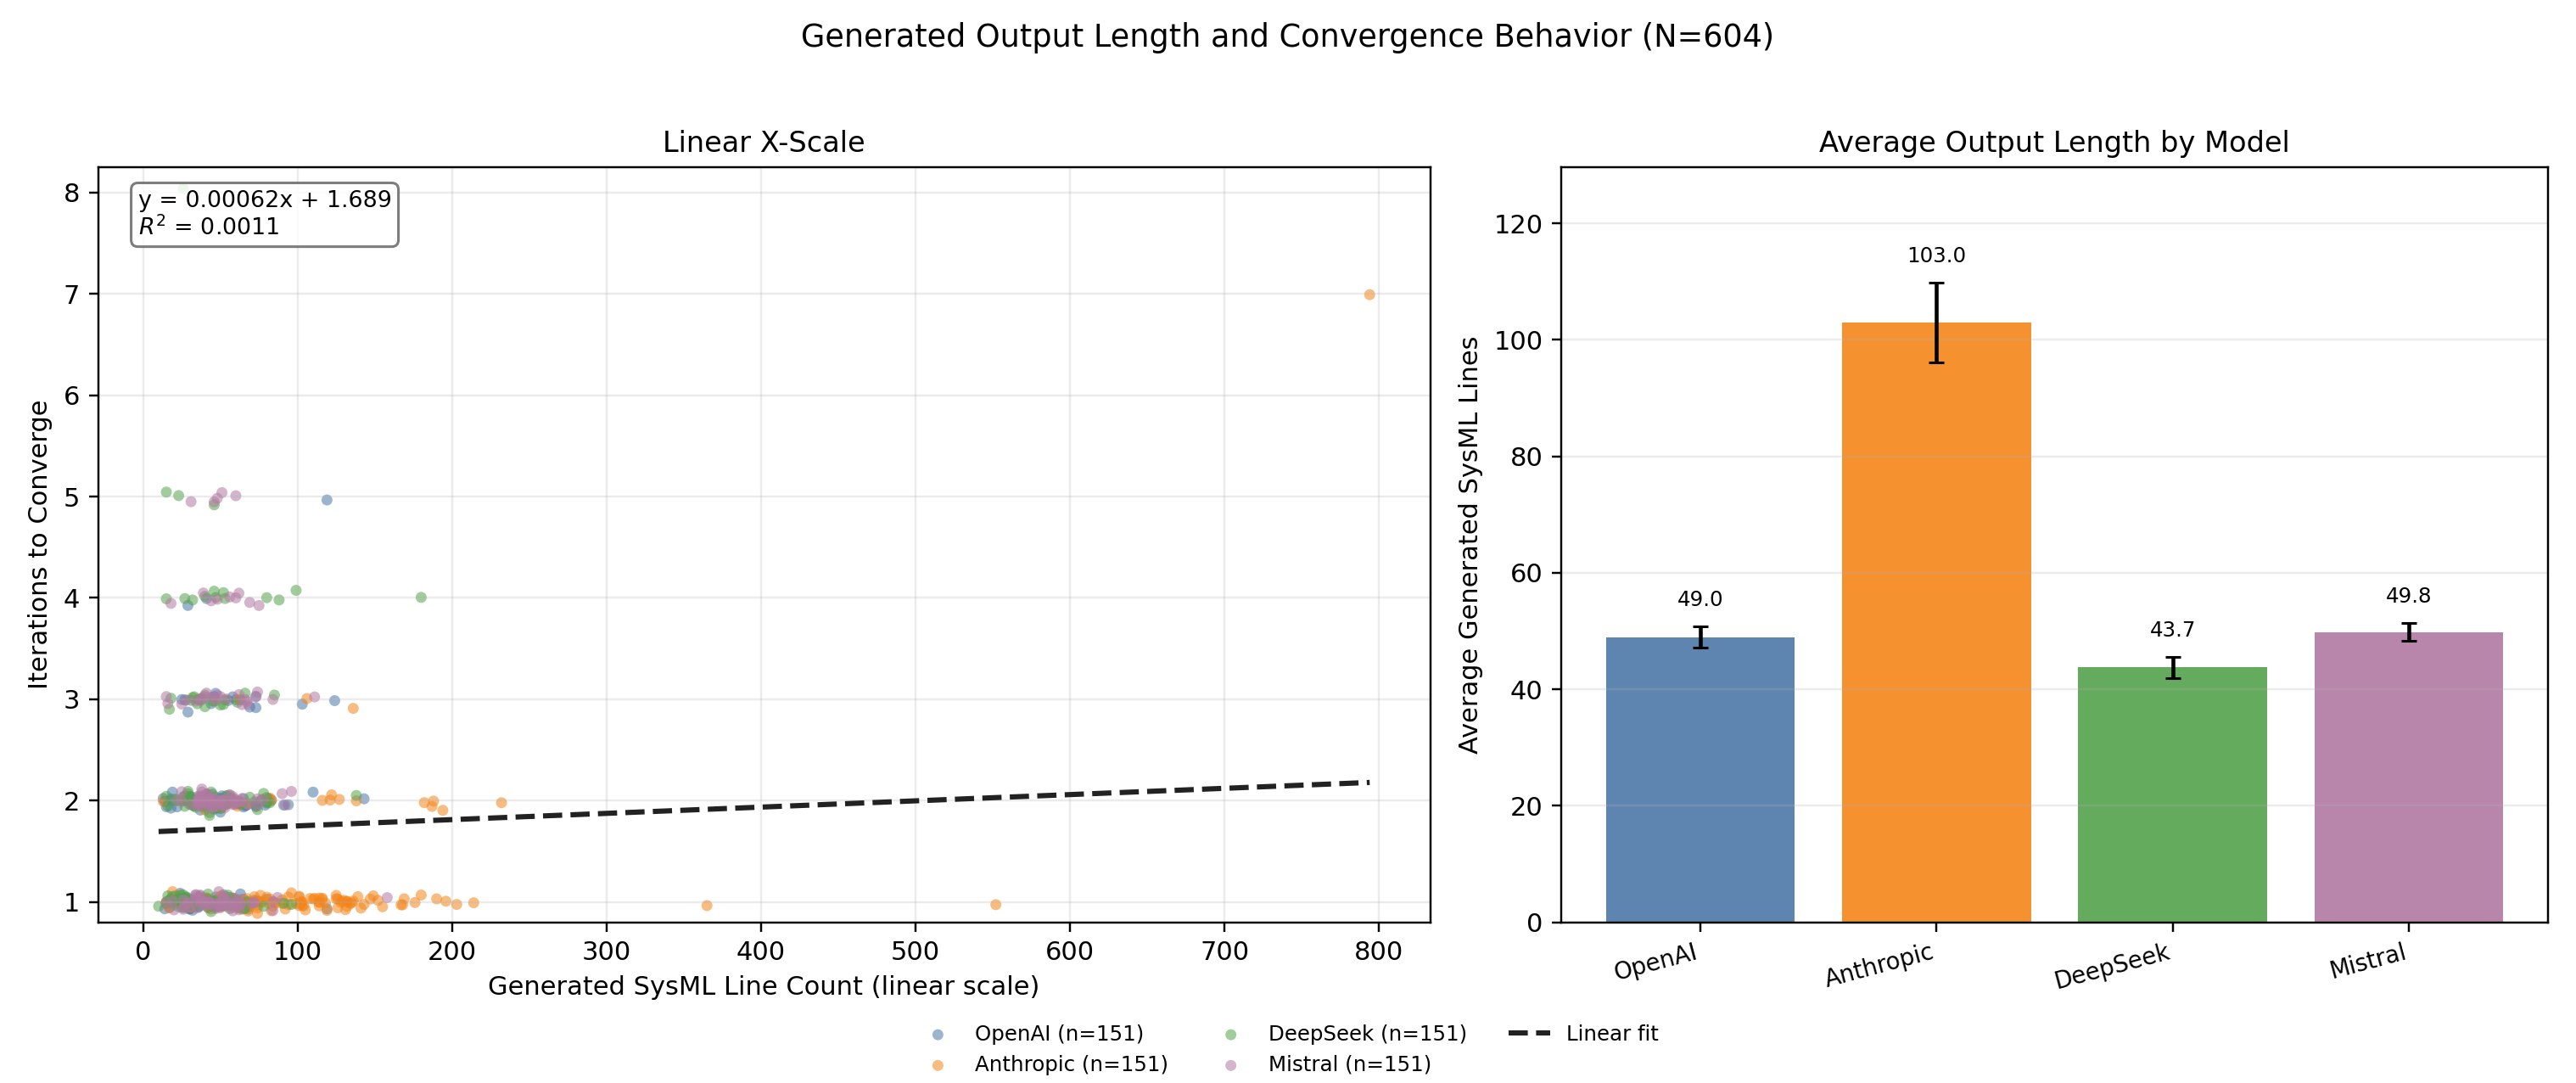
\includegraphics[width=\textwidth]{figures/fig14_generated_output_lines_vs_iterations_scatter_trend.png}
\caption{Generated SysML size analysis: linear-scale scatter of line count vs iterations-to-converge (with trendline and \(R^2\)) and average output length by model (\texttt{fig14}).}
\label{fig:fig14}
\end{figure}

\section{Error Analysis Using SysIDE Diagnostic Outputs}
Because eventual syntactic success is at ceiling, the key question shifts from \emph{whether} repairs happen to \emph{how} repair burden is distributed and how persistence behaves.

In this section, an \emph{error family} means the canonical diagnostic category emitted by the SysIDE compiler (e.g., \texttt{parsing-error}, \texttt{reference-error}). These family names are defined by SysIDE's diagnostic taxonomy and are used here as the primary unit for aggregation and persistence analysis.

\subsection{Where the Error Burden Concentrates}
Figure~\ref{fig:e15} compares single-shot error volume, cumulative all-iteration volume, and prompt coverage for top error families. The concentration is extreme: parsing-error and reference-error dominate both initial and cumulative burden.

Here, \emph{coverage across prompt set} means the number of distinct prompt IDs (out of 151 total prompts) for which a given error family appears at least once at any iteration (aggregated across all model runs).

Specifically, parsing-error contributes 1144 single-shot instances and 1666 cumulative instances across 126 prompts; reference-error contributes 824 single-shot and 1224 cumulative instances across 92 prompts. Together, these two families account for roughly 89\% of both single-shot and cumulative error instances.

\begin{figure}[H]
\centering
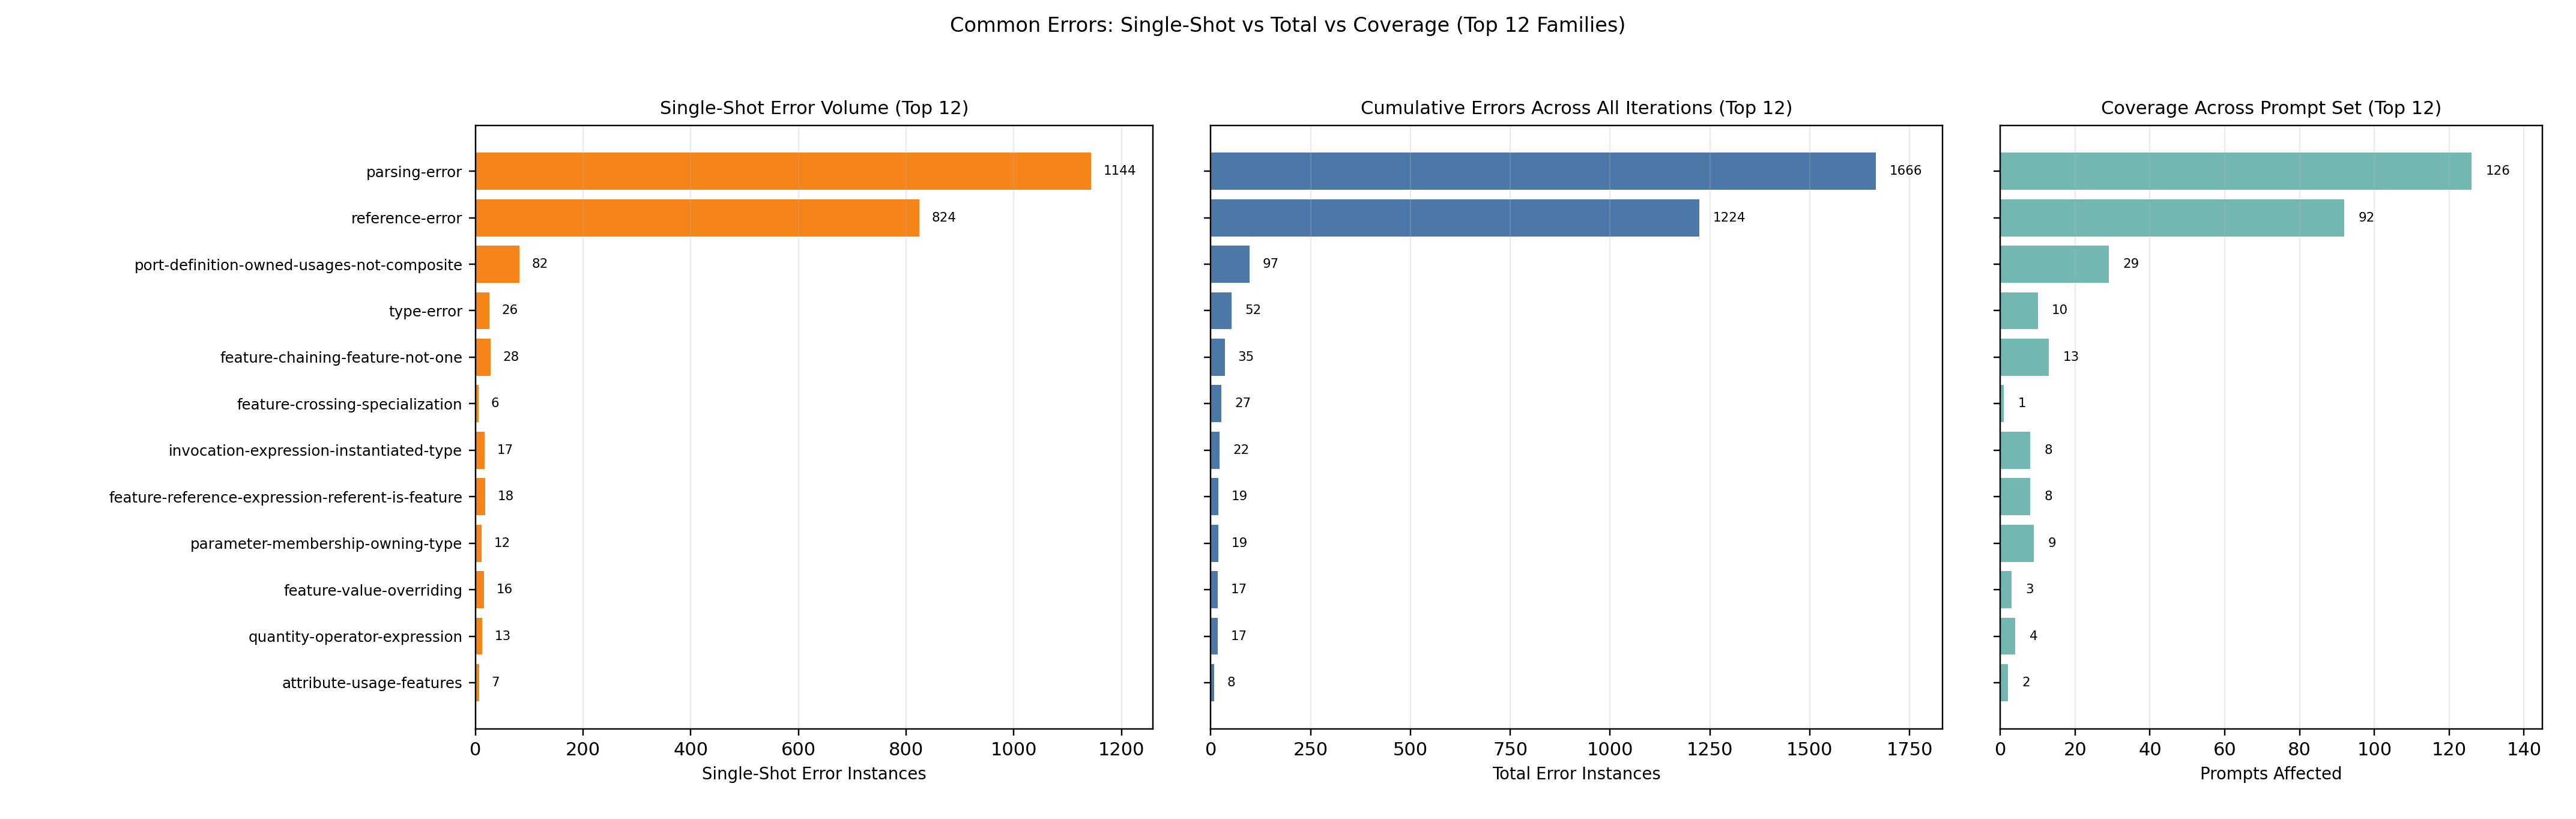
\includegraphics[width=\textwidth]{error_repair_insights/figures/figE15_common_errors_volume_and_coverage.png}
\caption{Single-shot volume, cumulative all-iteration volume, and coverage for top error families (\texttt{figE15}).}
\label{fig:e15}
\end{figure}

\subsection{How Quickly Common Errors Repair}
Figure~\ref{fig:e17} plots completion curves for the top-5 families by volume. Most episodes repair in one to two additional iterations, but the long tail is concentrated in the two dominant families.

For parsing-error, 71.255\% of episodes repair within one additional iteration and 89.879\% within two; 10.121\% require three or more. For reference-error, the corresponding values are 75.862\%, 93.793\%, and 6.207\%. In contrast, families such as port-definition-owned-usages-not-composite and type-error show no \( \geq 3 \)-iteration tail in this campaign.

\begin{figure}[H]
\centering
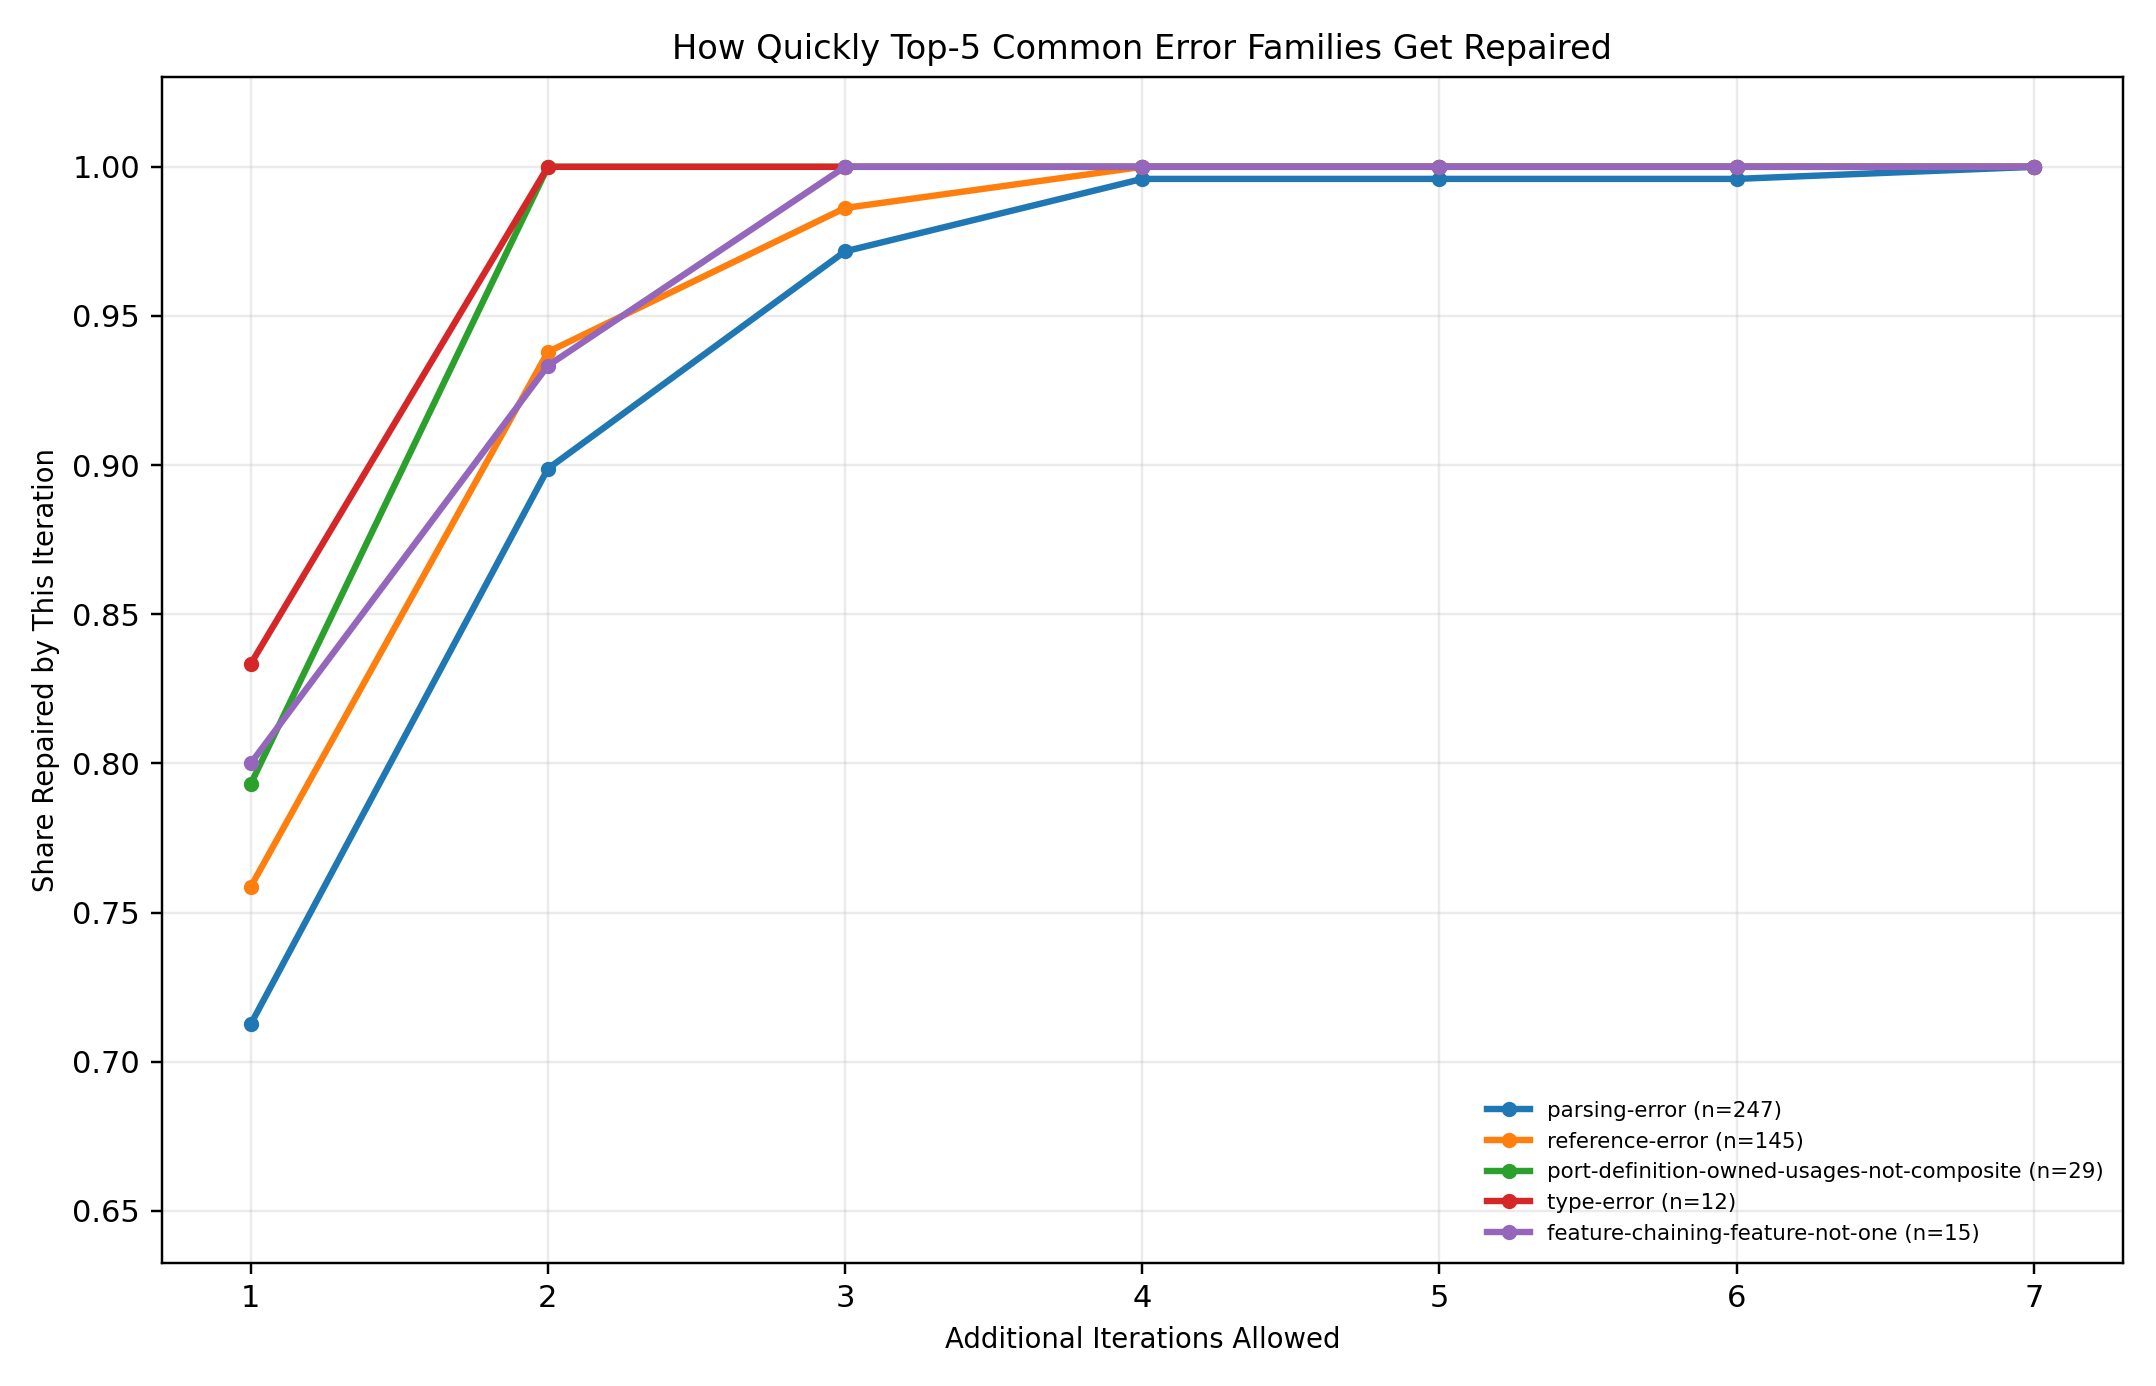
\includegraphics[width=\textwidth]{error_repair_insights/figures/figE17_repair_completion_curves_top_common.png}
\caption{Repair completion curves for top-5 error families (\texttt{figE17}).}
\label{fig:e17}
\end{figure}

\subsection{If an Error is Not Fixed Immediately, What Happens Next?}
In this note, a \emph{persistent error} is defined as an error-family episode that remains present for at least two consecutive iterations within the same run. This explicitly includes the case where the error appears in the single-shot output (iteration 1) and is still present after the first repair attempt (iteration 2).

To determine whether persistence is the ``same'' error versus only the same family label, we classify diagnostics at three levels:
\begin{itemize}
    \item \textbf{Exact recurrence}: same error family and same normalized diagnostic message recur across iterations.
    \item \textbf{Template recurrence}: exact message does not recur, but the same family-level diagnostic template recurs after normalizing variable details (e.g., quoted tokens or numeric literals).
    \item \textbf{Family-only churn}: the family recurs, but neither exact nor template-level recurrence is detected.
\end{itemize}
The persistence-mode percentages in Figure~\ref{fig:e18} are computed from this hierarchy (exact first, then template, then family-only).

Figure~\ref{fig:e18} characterizes persistence mode. Across persistent episodes, 84.8\% are repeated exact diagnostics, 8.0\% are same-template recurrences, and 7.2\% are family-only churn. This is important: persistence is usually not random error turnover, but repetition of the same unresolved diagnostic.

The family-level panel in Figure~\ref{fig:e18} shows this pattern is especially strong in the dominant families. Reference-error is 91.4\% exact recurrence among persistent episodes, while parsing-error is 78.9\% exact recurrence with a larger template/churn component.

\begin{figure}[H]
\centering
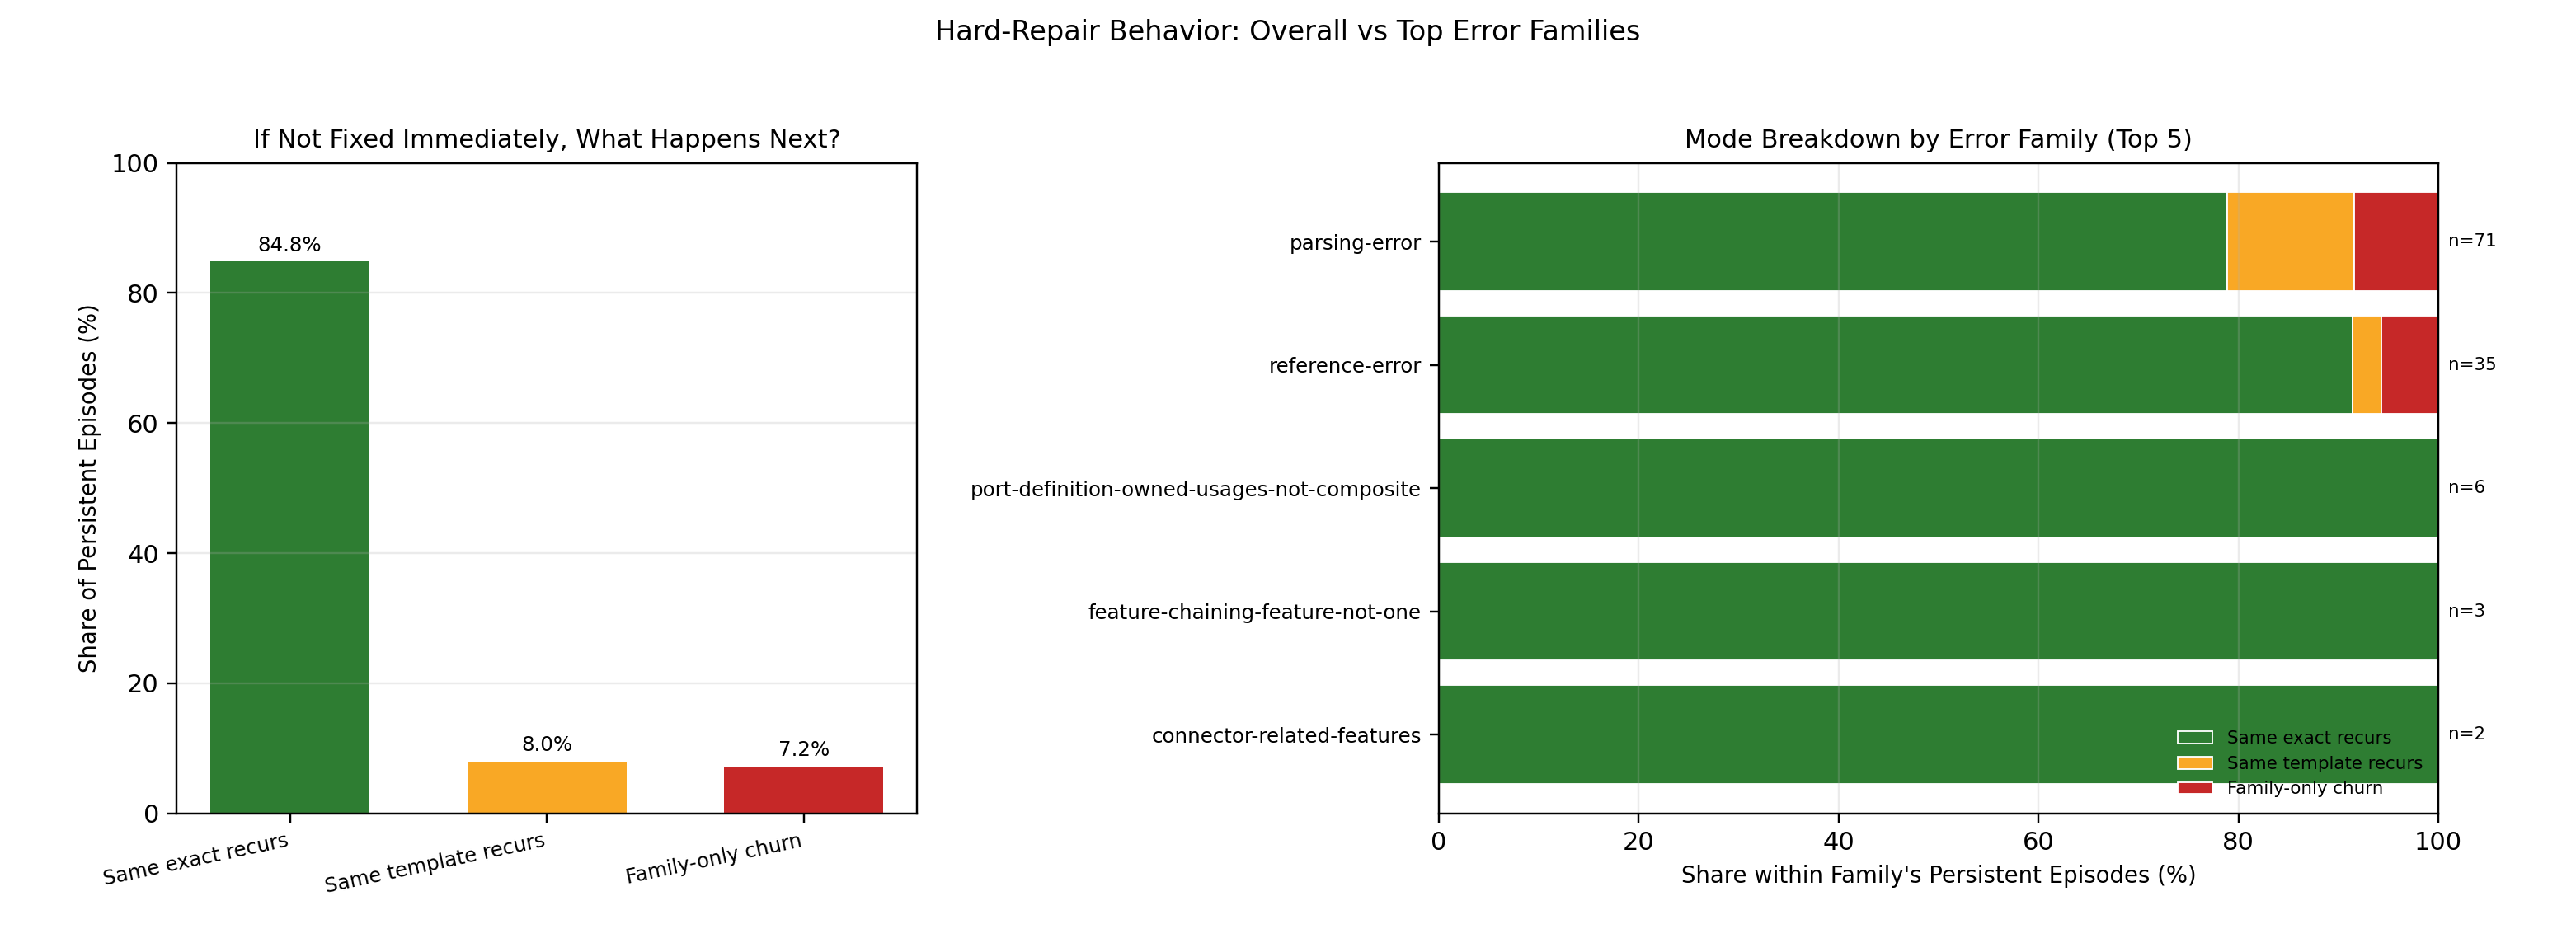
\includegraphics[width=\textwidth]{error_repair_insights/figures/figE18_unrepaired_status_and_persistence_behavior.png}
\caption{Persistence behavior overall and by top families (\texttt{figE18}).}
\label{fig:e18}
\end{figure}

\section{Chance's Interpretation}
I find it particularly interesting that SysML line count does not appear to be meaningfully correlated with the number of iterations required to reach syntactic correctness. We see this in two places: the generated-output size analysis (Figure~\ref{fig:fig14}) shows near-zero explanatory power for line count, and the SysMBench difficulty-stratified analysis (Figure~\ref{fig:fig09}) shows a similarly weak pattern across difficulty levels. Since SysMBench defines difficulty using line-count bins, this suggests that line-count-based difficulty is not a strong predictor of convergence effort in this compiler-in-the-loop setting.

\end{document}
